\documentclass{article}
\usepackage{pgfplots}
\pgfplotsset{compat=1.18}

\begin{document}

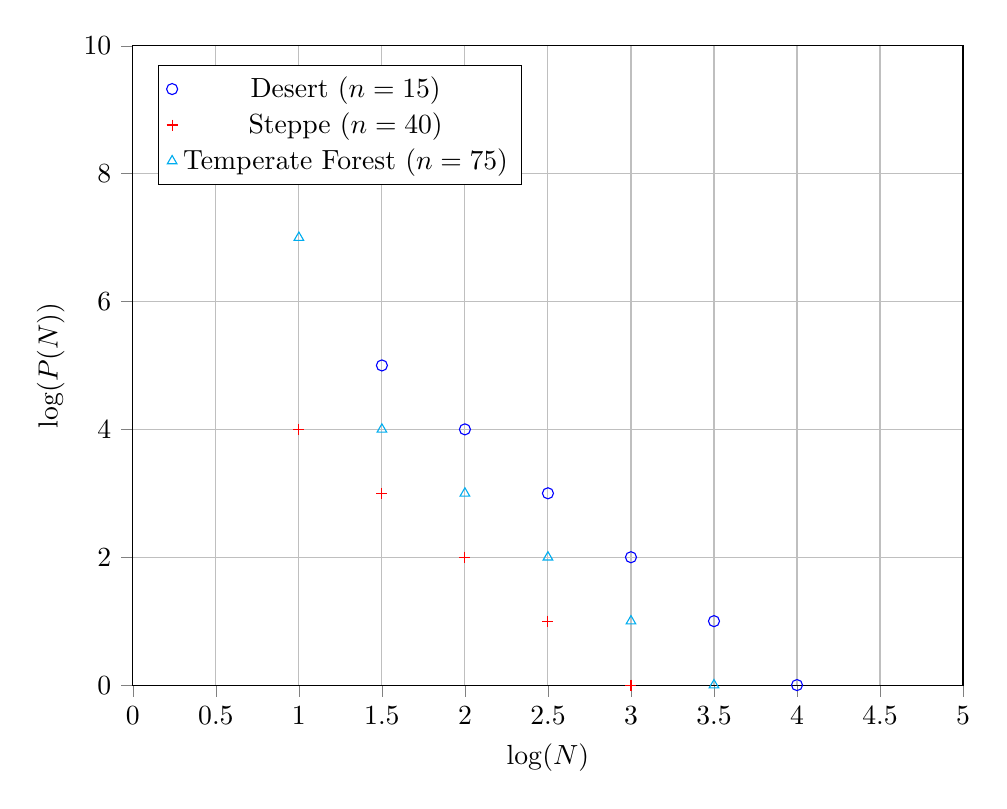
\begin{tikzpicture}
    \begin{axis}[
        xlabel=$\log(N)$,
        ylabel=$\log(P(N))$,
        xmin=0, xmax=5,
        ymin=0, ymax=10,
        legend pos=north west,
        log basis x={10},
        log basis y={10},
        grid=major,
        tick align=outside,
        tick pos=left,
        width=\textwidth,
        height=0.8*\textwidth,
        every axis plot/.append style={mark options={solid}},
    ]
    
    % Desert data
    \addplot[blue, only marks, mark=o] coordinates {
        (0.5, 9)
        (1, 8)
        (1.5, 5)
        (2, 4)
        (2.5, 3)
        (3, 2)
        (3.5, 1)
        (4, 0)
    };
    \addlegendentry{Desert ($n=15$)}
    
    % Steppe data
    \addplot[red, only marks, mark=+] coordinates {
        (1, 4)
        (1.5, 3)
        (2, 2)
        (2.5, 1)
        (3, 0)
        (3.5, -1)
        (4, -2)
        (4.5, -3)
    };
    \addlegendentry{Steppe ($n=40$)}
    
    % Temperate Forest data
    \addplot[cyan, only marks, mark=triangle] coordinates {
        (0.5, 8)
        (1, 7)
        (1.5, 4)
        (2, 3)
        (2.5, 2)
        (3, 1)
        (3.5, 0)
        (4, -1)
        (4.5, -2)
    };
    \addlegendentry{Temperate Forest ($n=75$)}
    
    \end{axis}
\end{tikzpicture}

\end{document}